\documentclass{article.cls}
\usepackage{tikz}
\usetikzlibrary{shapes, arrows.meta, positioning, fit, backgrounds}
\usepackage{enumitem}
\usepackage{xcolor}
\usepackage{listings}
\usepackage{color}
\usepackage{textcomp}

\definecolor{codegreen}{rgb}{0,0.6,0}
\definecolor{codegray}{rgb}{0.5,0.5,0.5}
\definecolor{codepurple}{rgb}{0.58,0,0.82}

\lstset{
    basicstyle=\ttfamily\footnotesize,
    breaklines=true,
    frame=single,
    numbers=left,
    numberstyle=\tiny\color{codegray},
    keywordstyle=\color{blue},
    commentstyle=\color{codegreen},
    stringstyle=\color{codepurple}
}

\begin{document}

    \title{DOM Events: Complete Guide with Diagrams}
    \author{Web Development Course}
    \date{}
    \maketitle

    \section*{Part 1: The Fundamentals of Events}

    \subsection*{What is a DOM Event? The "Doorbell" Analogy}

    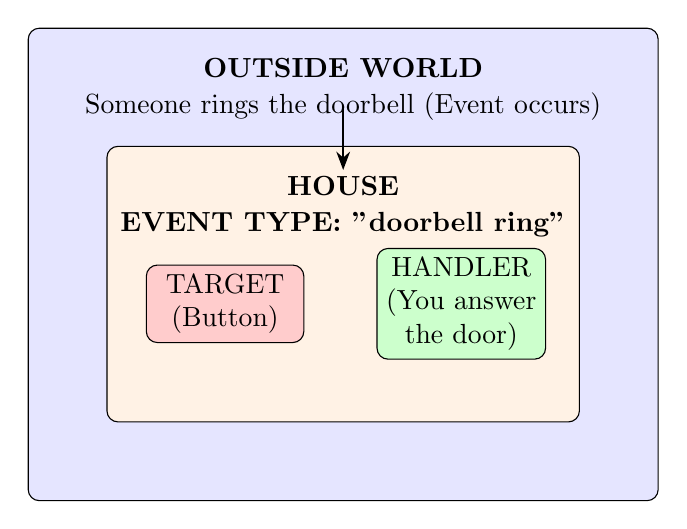
\begin{tikzpicture}[
        box/.style={draw, rounded corners, align=center, minimum width=2cm},
        arrow/.style={-Stealth, thick}
    ]
        % Outside area
        \draw[rounded corners, fill=blue!10] (0,0) rectangle (8,6);
        \node at (4,5.5) {\textbf{OUTSIDE WORLD}};
        \node at (4,5) {Someone rings the doorbell (Event occurs)};

        % House
        \draw[rounded corners, fill=orange!10] (1,1) rectangle (7,4.5);
        \node at (4,4) {\textbf{HOUSE}};

        % Target and Handler
        \node[box, fill=red!20] (target) at (2.5,2.5) {TARGET\\ (Button)};
        \node[box, fill=green!20] (handler) at (5.5,2.5) {HANDLER\\ (You answer\\ the door)};

        % Event Type
        \node at (4,3.5) {\textbf{EVENT TYPE: "doorbell ring"}};

        % Arrows
        \draw[arrow] (4,5) -- (4,4.2);
    \end{tikzpicture}

    \subsection*{Modern Event Handling with \texttt{addEventListener}}

    \begin{lstlisting}[language=JavaScript, caption=Modern Event Handling]
// OLD WAY (not recommended - separation of concerns)
<button onclick="handleClick()">Click me</button>

// MODERN WAY
const button = document.querySelector('button');
button.addEventListener('click', function(event) {
    // event object contains all information
    console.log(event.target);      // The button element
    console.log(event.type);        // 'click'
    console.log(event.clientX);     // Mouse position X
});
    \end{lstlisting}

    \subsection*{The Event Object - Information Packet}

    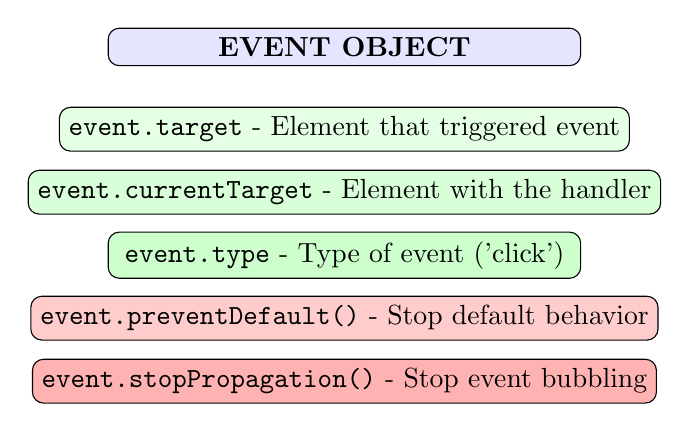
\begin{tikzpicture}[
        nested/.style={draw, rounded corners, align=center, minimum width=6cm},
        inner/.style={draw, rounded corners, align=center, minimum width=5.5cm}
    ]
        % Outer box
        \node[nested, fill=blue!10] (outer) {\textbf{EVENT OBJECT}};

        % Nested boxes
        \node[nested, fill=green!10, yshift=-0.8cm] (target) at (outer.south)
            {\texttt{event.target} - Element that triggered event};

        \node[nested, fill=green!15, yshift=-1.6cm] (current) at (outer.south)
            {\texttt{event.currentTarget} - Element with the handler};

        \node[nested, fill=green!20, yshift=-2.4cm] (type) at (outer.south)
            {\texttt{event.type} - Type of event ('click')};

        \node[nested, fill=red!20, yshift=-3.2cm] (prevent) at (outer.south)
            {\texttt{event.preventDefault()} - Stop default behavior};

        \node[nested, fill=red!30, yshift=-4cm] (stop) at (outer.south)
            {\texttt{event.stopPropagation()} - Stop event bubbling};
    \end{tikzpicture}

    \section*{Part 2: The Three Phases of an Event}

    \subsection*{Event Flow Visualization}

    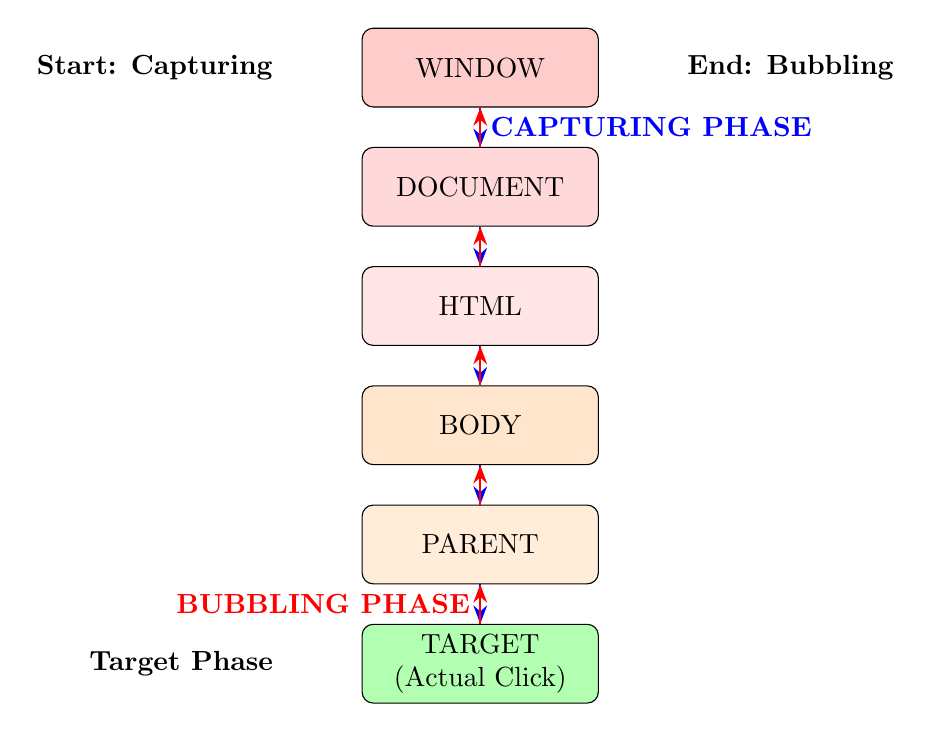
\begin{tikzpicture}[
        phase/.style={draw, rounded corners, align=center, minimum height=1cm, minimum width=3cm},
        arrow/.style={-Stealth, thick, blue},
        label/.style={align=center}
    ]

        % Define nodes for event flow
        \node[phase, fill=red!20] (window) {WINDOW};
        \node[phase, fill=red!15, below=0.5cm of window] (document) {DOCUMENT};
        \node[phase, fill=red!10, below=0.5cm of document] (html) {HTML};
        \node[phase, fill=orange!20, below=0.5cm of html] (body) {BODY};
        \node[phase, fill=orange!15, below=0.5cm of body] (parent) {PARENT};
        \node[phase, fill=green!30, below=0.5cm of parent] (target) {TARGET \\ (Actual Click)};

        % Capturing phase arrow
        \draw[arrow] (window.south) -- node[right] {\textbf{CAPTURING PHASE}} (document.north);
        \draw[arrow] (document.south) -- (html.north);
        \draw[arrow] (html.south) -- (body.north);
        \draw[arrow] (body.south) -- (parent.north);
        \draw[arrow] (parent.south) -- (target.north);

        % Bubbling phase arrow
        \draw[arrow, red] (target.north) -- node[left] {\textbf{BUBBLING PHASE}} (parent.south);
        \draw[arrow, red] (parent.north) -- (body.south);
        \draw[arrow, red] (body.north) -- (html.south);
        \draw[arrow, red] (html.north) -- (document.south);
        \draw[arrow, red] (document.north) -- (window.south);

        % Labels
        \node[label, left=1cm of window] {\textbf{Start: Capturing}};
        \node[label, left=1cm of target] {\textbf{Target Phase}};
        \node[label, right=1cm of window] {\textbf{End: Bubbling}};

    \end{tikzpicture}

    \subsection*{Controlling Event Flow}

    \begin{lstlisting}[language=JavaScript, caption=Event Flow Control]
// Stop event from propagating further
element.addEventListener('click', function(event) {
    event.stopPropagation(); // Prevents bubbling/capturing
    // event.stopImmediatePropagation() - stops all handlers
});

// Use capturing phase (instead of bubbling)
element.addEventListener('click', handler, true);
// OR
element.addEventListener('click', handler, {capture: true});

// Example with all phases
parent.addEventListener('click', function(event) {
    console.log('Capturing phase - parent');
}, true);

parent.addEventListener('click', function(event) {
    console.log('Bubbling phase - parent');
});
    \end{lstlisting}

    \section*{Part 3: Event Delegation Pattern}

    \subsection*{Why Event Delegation?}

    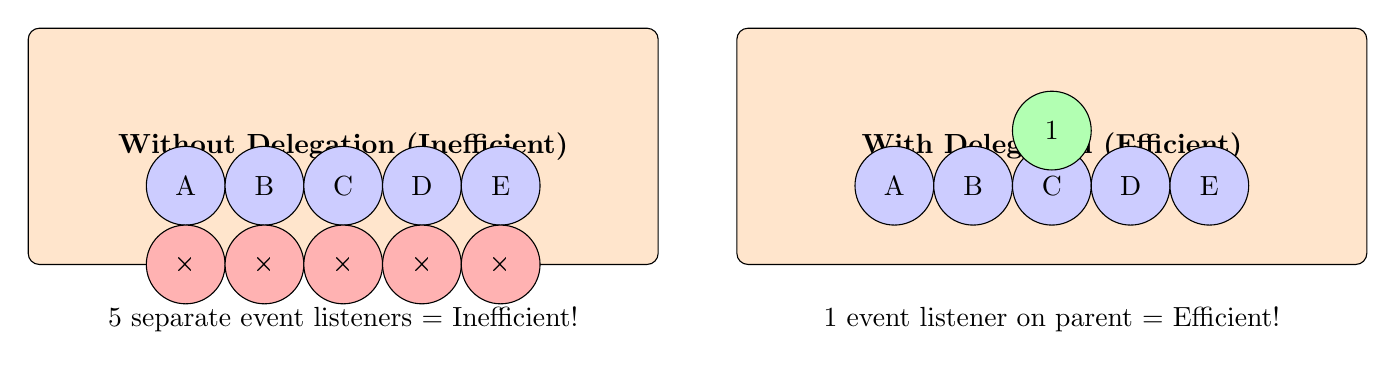
\begin{tikzpicture}[
        item/.style={draw, circle, fill=blue!20, minimum size=1cm},
        parent/.style={draw, rounded corners, fill=orange!20, minimum width=8cm, minimum height=3cm}
    ]

        % Without delegation
        \node[parent] (without) at (0,0) {\textbf{Without Delegation (Inefficient)}};

        \node[item] (a1) at (-2, -0.5) {A};
        \node[item] (b1) at (-1, -0.5) {B};
        \node[item] (c1) at (0, -0.5) {C};
        \node[item] (d1) at (1, -0.5) {D};
        \node[item] (e1) at (2, -0.5) {E};

        \node[item, fill=red!30] (x1) at (-2, -1.5) {\texttimes};
        \node[item, fill=red!30] (x2) at (-1, -1.5) {\texttimes};
        \node[item, fill=red!30] (x3) at (0, -1.5) {\texttimes};
        \node[item, fill=red!30] (x4) at (1, -1.5) {\texttimes};
        \node[item, fill=red!30] (x5) at (2, -1.5) {\texttimes};

        \node at (0, -2.2) {5 separate event listeners = Inefficient!};

        % With delegation
        \node[parent] (with) at (9,0) {\textbf{With Delegation (Efficient)}};

        \node[item] (a2) at (7, -0.5) {A};
        \node[item] (b2) at (8, -0.5) {B};
        \node[item] (c2) at (9, -0.5) {C};
        \node[item] (d2) at (10, -0.5) {D};
        \node[item] (e2) at (11, -0.5) {E};

        \node[item, fill=green!30, yshift=0.7cm] (single) at (9, -0.5) {1};

        \node at (9, -2.2) {1 event listener on parent = Efficient!};

    \end{tikzpicture}

    \subsection*{\texttt{event.target} vs \texttt{event.currentTarget}}

    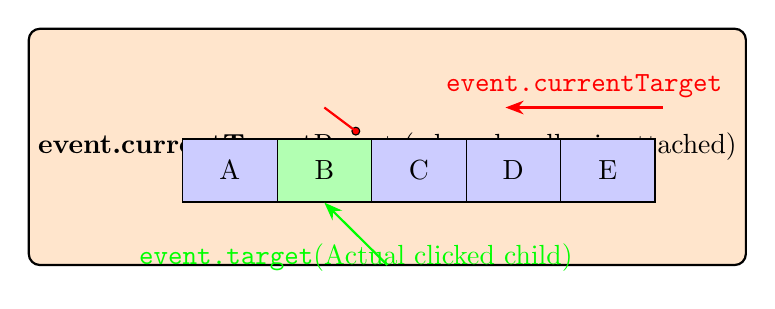
\begin{tikzpicture}[
        item/.style={draw, rectangle, fill=blue!20, minimum width=1.2cm, minimum height=0.8cm},
        parent/.style={draw, thick, rounded corners, fill=orange!20, minimum width=8cm, minimum height=3cm}
    ]

        % Parent container
        \node[parent] (parent) {\textbf{event.currentTarget} \\ Parent (where handler is attached)};

        % Child items
        \node[item] (an) at (-2, -0.3) {A};
        \node[item, fill=green!30] (b) at (-0.8, -0.3) {B};
        \node[item] (c) at (0.4, -0.3) {C};
        \node[item] (d) at (1.6, -0.3) {D};
        \node[item] (e) at (2.8, -0.3) {E};

        % Labels and arrows
        \draw[-Stealth, thick, red] (3.5, 0.5) -- node[above] {\texttt{event.currentTarget}} (1.5, 0.5);
        \draw[-Stealth, thick, green] (0, -1.5) -- node[below] {\texttt{event.target} \\ (Actual clicked child)} (b.south);

        % Click indicator
        \node[draw, circle, fill=red, inner sep=1pt] at (-0.4, 0.2) {};
        \draw[red, thick] (-0.8, 0.5) -- (-0.4, 0.2);

    \end{tikzpicture}

    \subsection*{Practical Example: Dynamic List with Event Delegation}

    \begin{lstlisting}[language=HTML, caption=HTML Structure]
<ul id="shoppingList">
    <li data-id="1">Milk</li>
    <li data-id="2">Bread</li>
    <li data-id="3">Eggs</li>
</ul>
<button onclick="addItem('Butter')">Add Butter</button>
    \end{lstlisting}

    \begin{lstlisting}[language=JavaScript, caption=Event Delegation Implementation]
// SINGLE event listener for ALL items (present and future)
document.getElementById('shoppingList').addEventListener('click', function(event) {
    // event.target = the actual <li> that was clicked
    // event.currentTarget = the <ul> (this)
    
    if (event.target.tagName === 'LI') {
        const itemId = event.target.dataset.id;
        const itemText = event.target.textContent;
        console.log(`Clicked item ${itemId}: ${itemText}`);
        
        // Remove the clicked item
        event.target.remove();
    }
});

// Add new items dynamically - they automatically work!
function addItem(text) {
    const list = document.getElementById('shoppingList');
    const li = document.createElement('li');
    li.textContent = text;
    li.dataset.id = Date.now(); // Unique ID
    list.appendChild(li);
    // No need to add event listener - delegation handles it!
}

// New items added later will automatically work with the existing listener
setTimeout(() => addItem('Cheese'), 5000);
    \end{lstlisting}

    \subsection*{Benefits of Event Delegation}

    \begin{itemize}
        \item \textbf{Memory Efficient}: One listener instead of many
        \item \textbf{Dynamic Content}: Works with elements added later
        \item \textbf{Cleaner Code}: Centralized event handling
        \item \textbf{Better Performance}: Fewer event listeners to manage
        \item \textbf{Easier Maintenance}: One place to manage event logic
    \end{itemize}

\end{document}